\documentclass[a4paper, 12pt, oneside, twocolumn]{article}
\usepackage[nf]{coelacanth}
\usepackage[T1]{fontenc}
\usepackage{booktabs}
\usepackage{textalpha}
\usepackage{url}
\setlength{\emergencystretch}{15pt}
\usepackage{fancyhdr}
\usepackage{amssymb}
\usepackage{lscape}
\usepackage{longtable}
\usepackage{tablefootnote}
\usepackage{array}
\usepackage{imakeidx}
\usepackage{float}
\usepackage{qtree}
\usepackage{microtype}
\usepackage[dvipsnames]{xcolor}
\usepackage{eso-pic,graphicx}
\usepackage[top=38mm, bottom=33mm, outer=21mm, inner=21mm]{geometry}
\setlength{\columnsep}{90pt}
\def\arraystretch{1.25}
\usepackage{setspace}
\onehalfspacing
% change color of text, example replace all \color{Goldenrod} with \color{lightgray}
\definecolor{customColor}{RGB}{231, 229, 232}

\makeatletter % change only the display of \thepage, but not \thepage itself:
\patchcmd{\ps@plain}{\thepage}{\bfseries\large\color{customColor}{\thepage}}{}{}
\makeatother

\color{customColor}
\begin{document}
\bfseries
\renewcommand{\thefigure}{\bfseries{\arabic{figure}}}
\renewcommand\thefootnote{\bfseries{\arabic{footnote}}}
\let\oldfootnote\footnote
    \renewcommand{\footnote}[1]{\oldfootnote{\bfseries#1}}

\pagestyle{plain} % after changing a pagestyle command, it's necessary to invoke it explicitly
\AddToShipoutPictureBG*{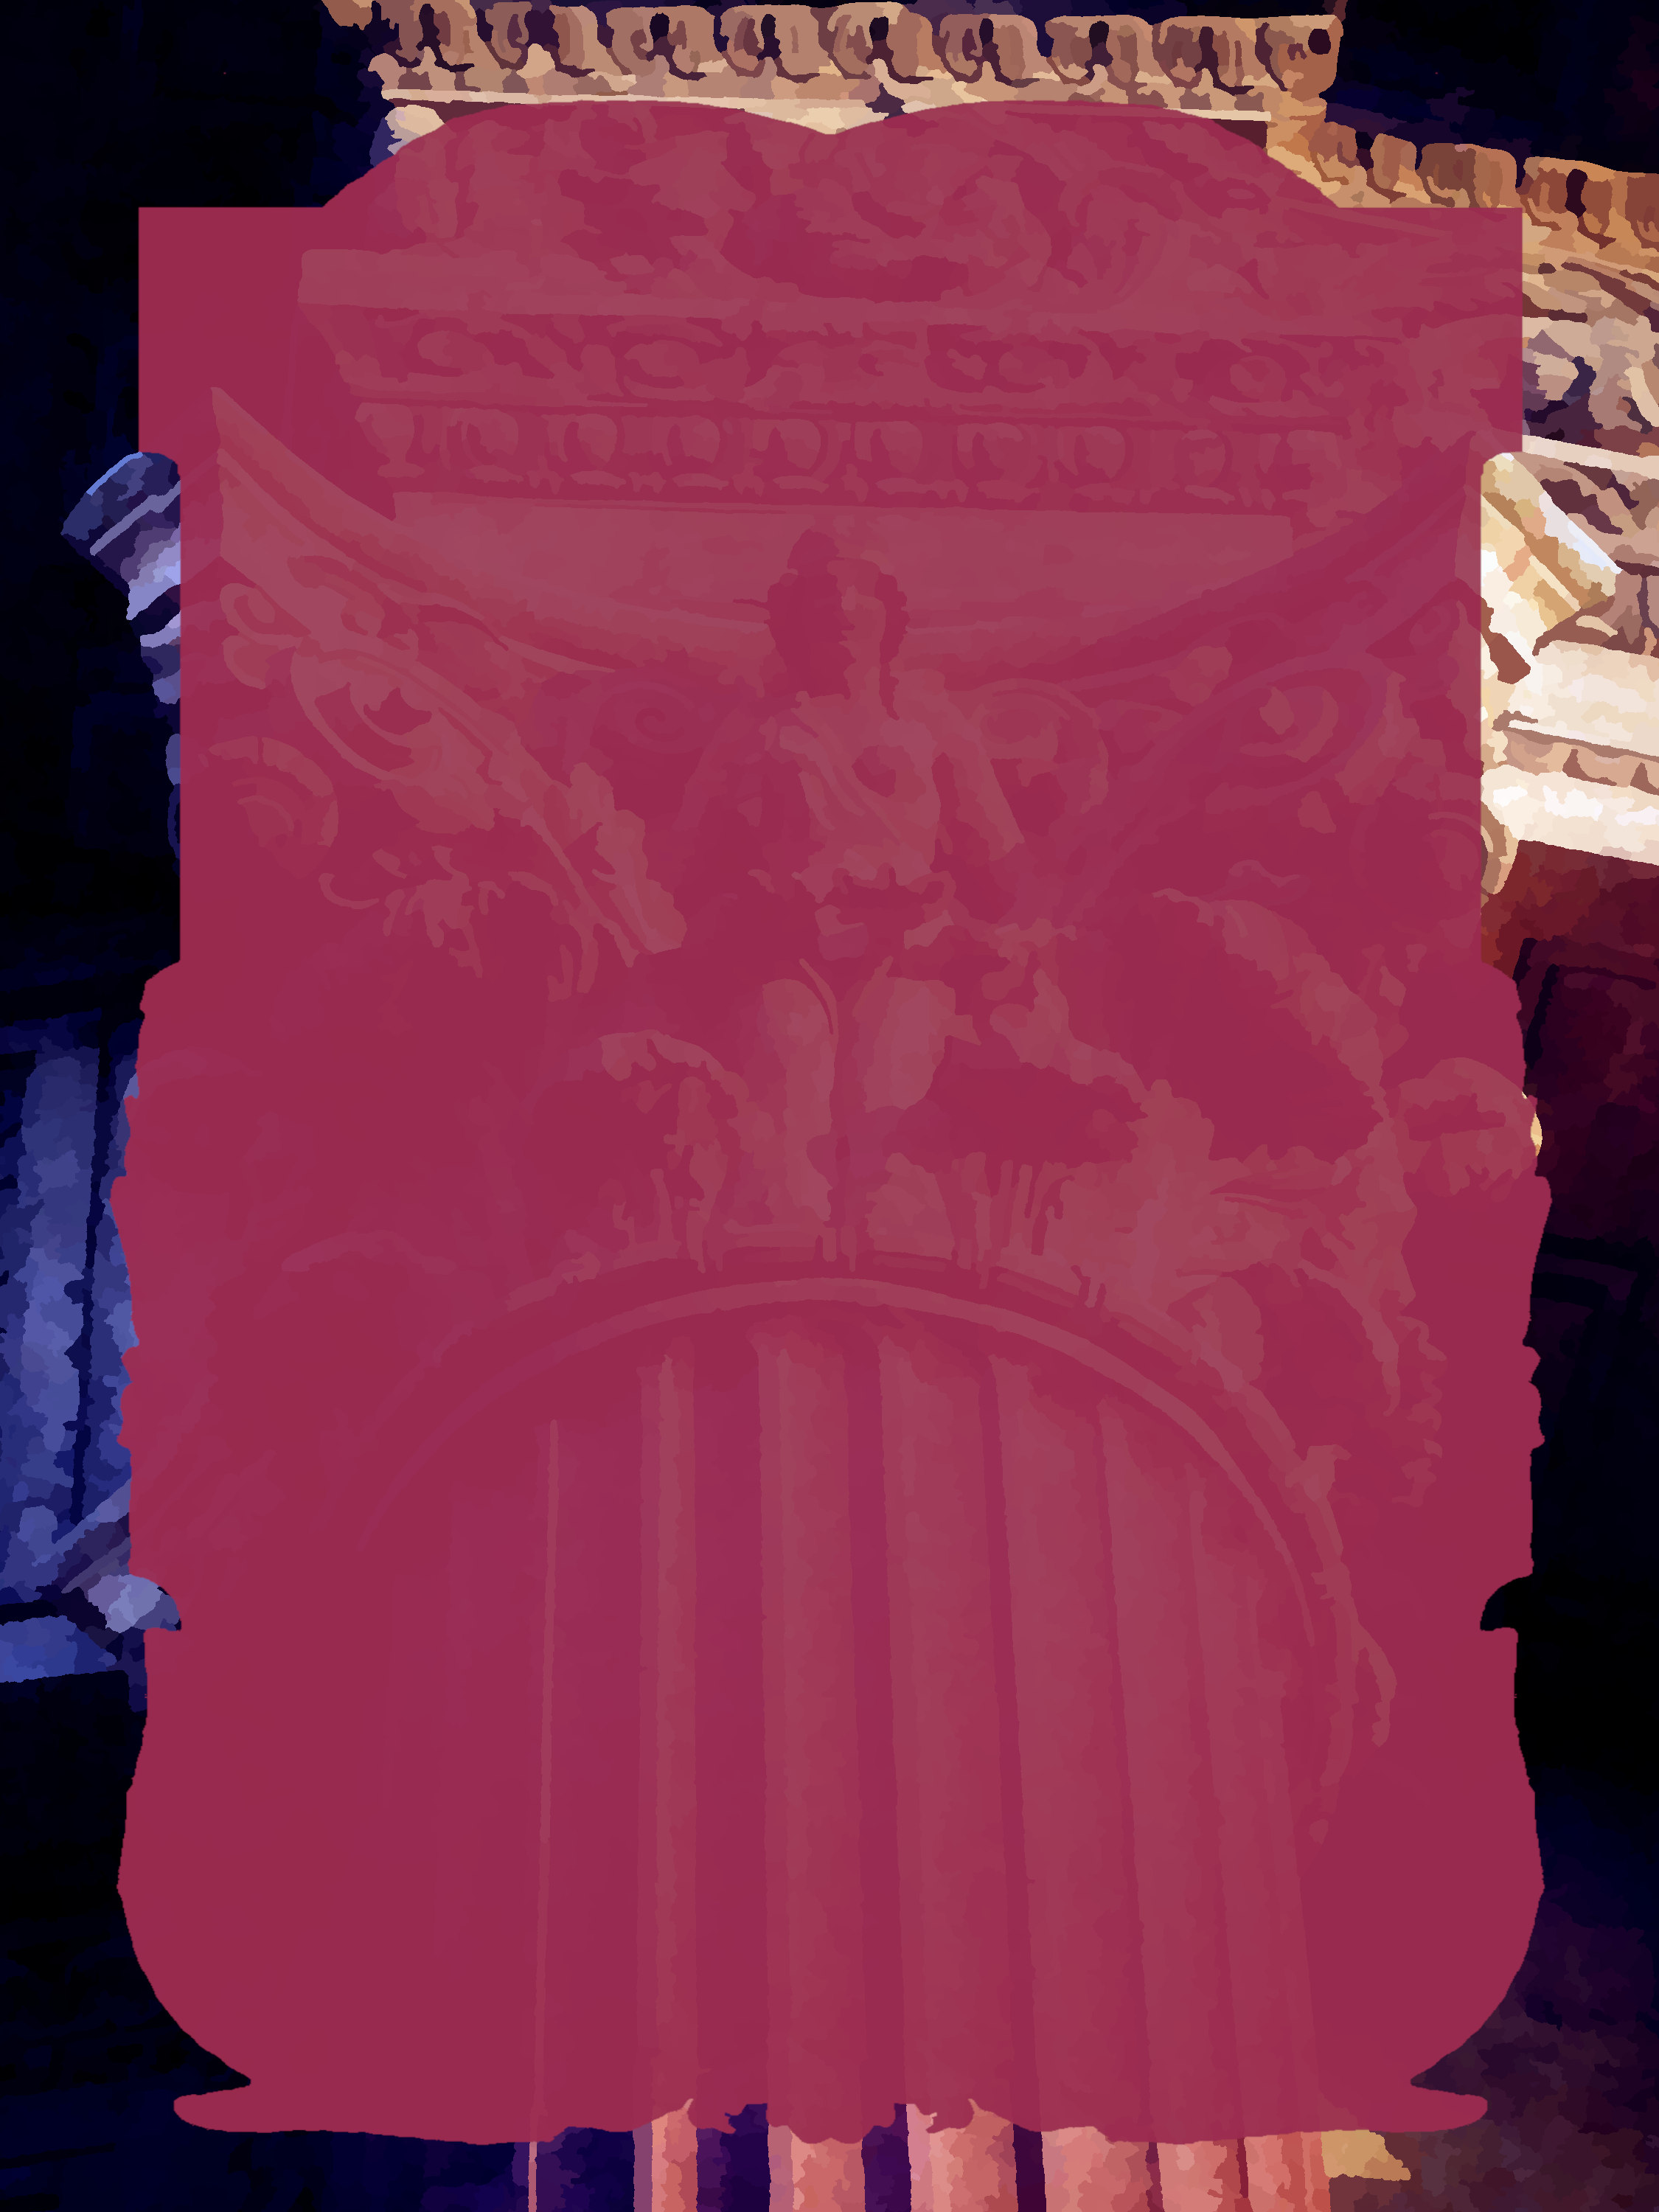
\includegraphics[width=\paperwidth,height=\paperheight]{columnfull96.jpeg}}
\begin{titlepage} % Suppresses headers and footers on the title page
	\centering % Centre everything on the title page
	\scshape % Use small caps for all text on the title page

	%------------------------------------------------
	%	Title
	%------------------------------------------------
	
	\rule{0.8\textwidth}{1.6pt}\vspace*{-\baselineskip}\vspace*{2pt} % Thick horizontal rule
	\rule{0.8\textwidth}{0.4pt} % Thin horizontal rule
	
	\vspace{0.75\baselineskip} % Whitespace above the title

        {\LARGE Experiments and Observations on\\ certain stony and metalline\\ Substances,\\ which at different Times\\ are said to have fallen on the Earth;\\ also on\\ various Kinds of native Iron.} % Title
	
	\vspace{0.75\baselineskip} % Whitespace below the title
	
	\rule{0.8\textwidth}{0.4pt}\vspace*{-\baselineskip}\vspace{3.2pt} % Thin horizontal rule
	\rule{0.8\textwidth}{1.6pt} % Thick horizontal rule
	
	\vspace{1\baselineskip} % Whitespace after the title block
	
	%------------------------------------------------
	%	Subtitle
	%------------------------------------------------
	
	{\scshape\Large By Edward Howard, \emph{Esq. FRS}} % Subtitle or further description
	
	\vspace*{1\baselineskip} % Whitespace under the subtitle
	
	%------------------------------------------------
	%	Editor(s)
	%------------------------------------------------

	\vspace{1\baselineskip} % Whitespace before the editors

    %------------------------------------------------
	%	Cover photo
	%------------------------------------------------
	
	%\includegraphics[scale=1]{cover}
	
	%------------------------------------------------
	%	Publisher
	%------------------------------------------------
		
	\vspace*{\fill}% Whitespace under the publisher logo
	
	1802.% Publication year
	
	\vspace{1\baselineskip} % Whitespace under the publisher logo

        Internet Archive Online Edition  % Publication year
	
	{\small Attribution NonCommercial ShareAlike 4.0 International } % Publisher
\end{titlepage}
\AddToShipoutPictureBG{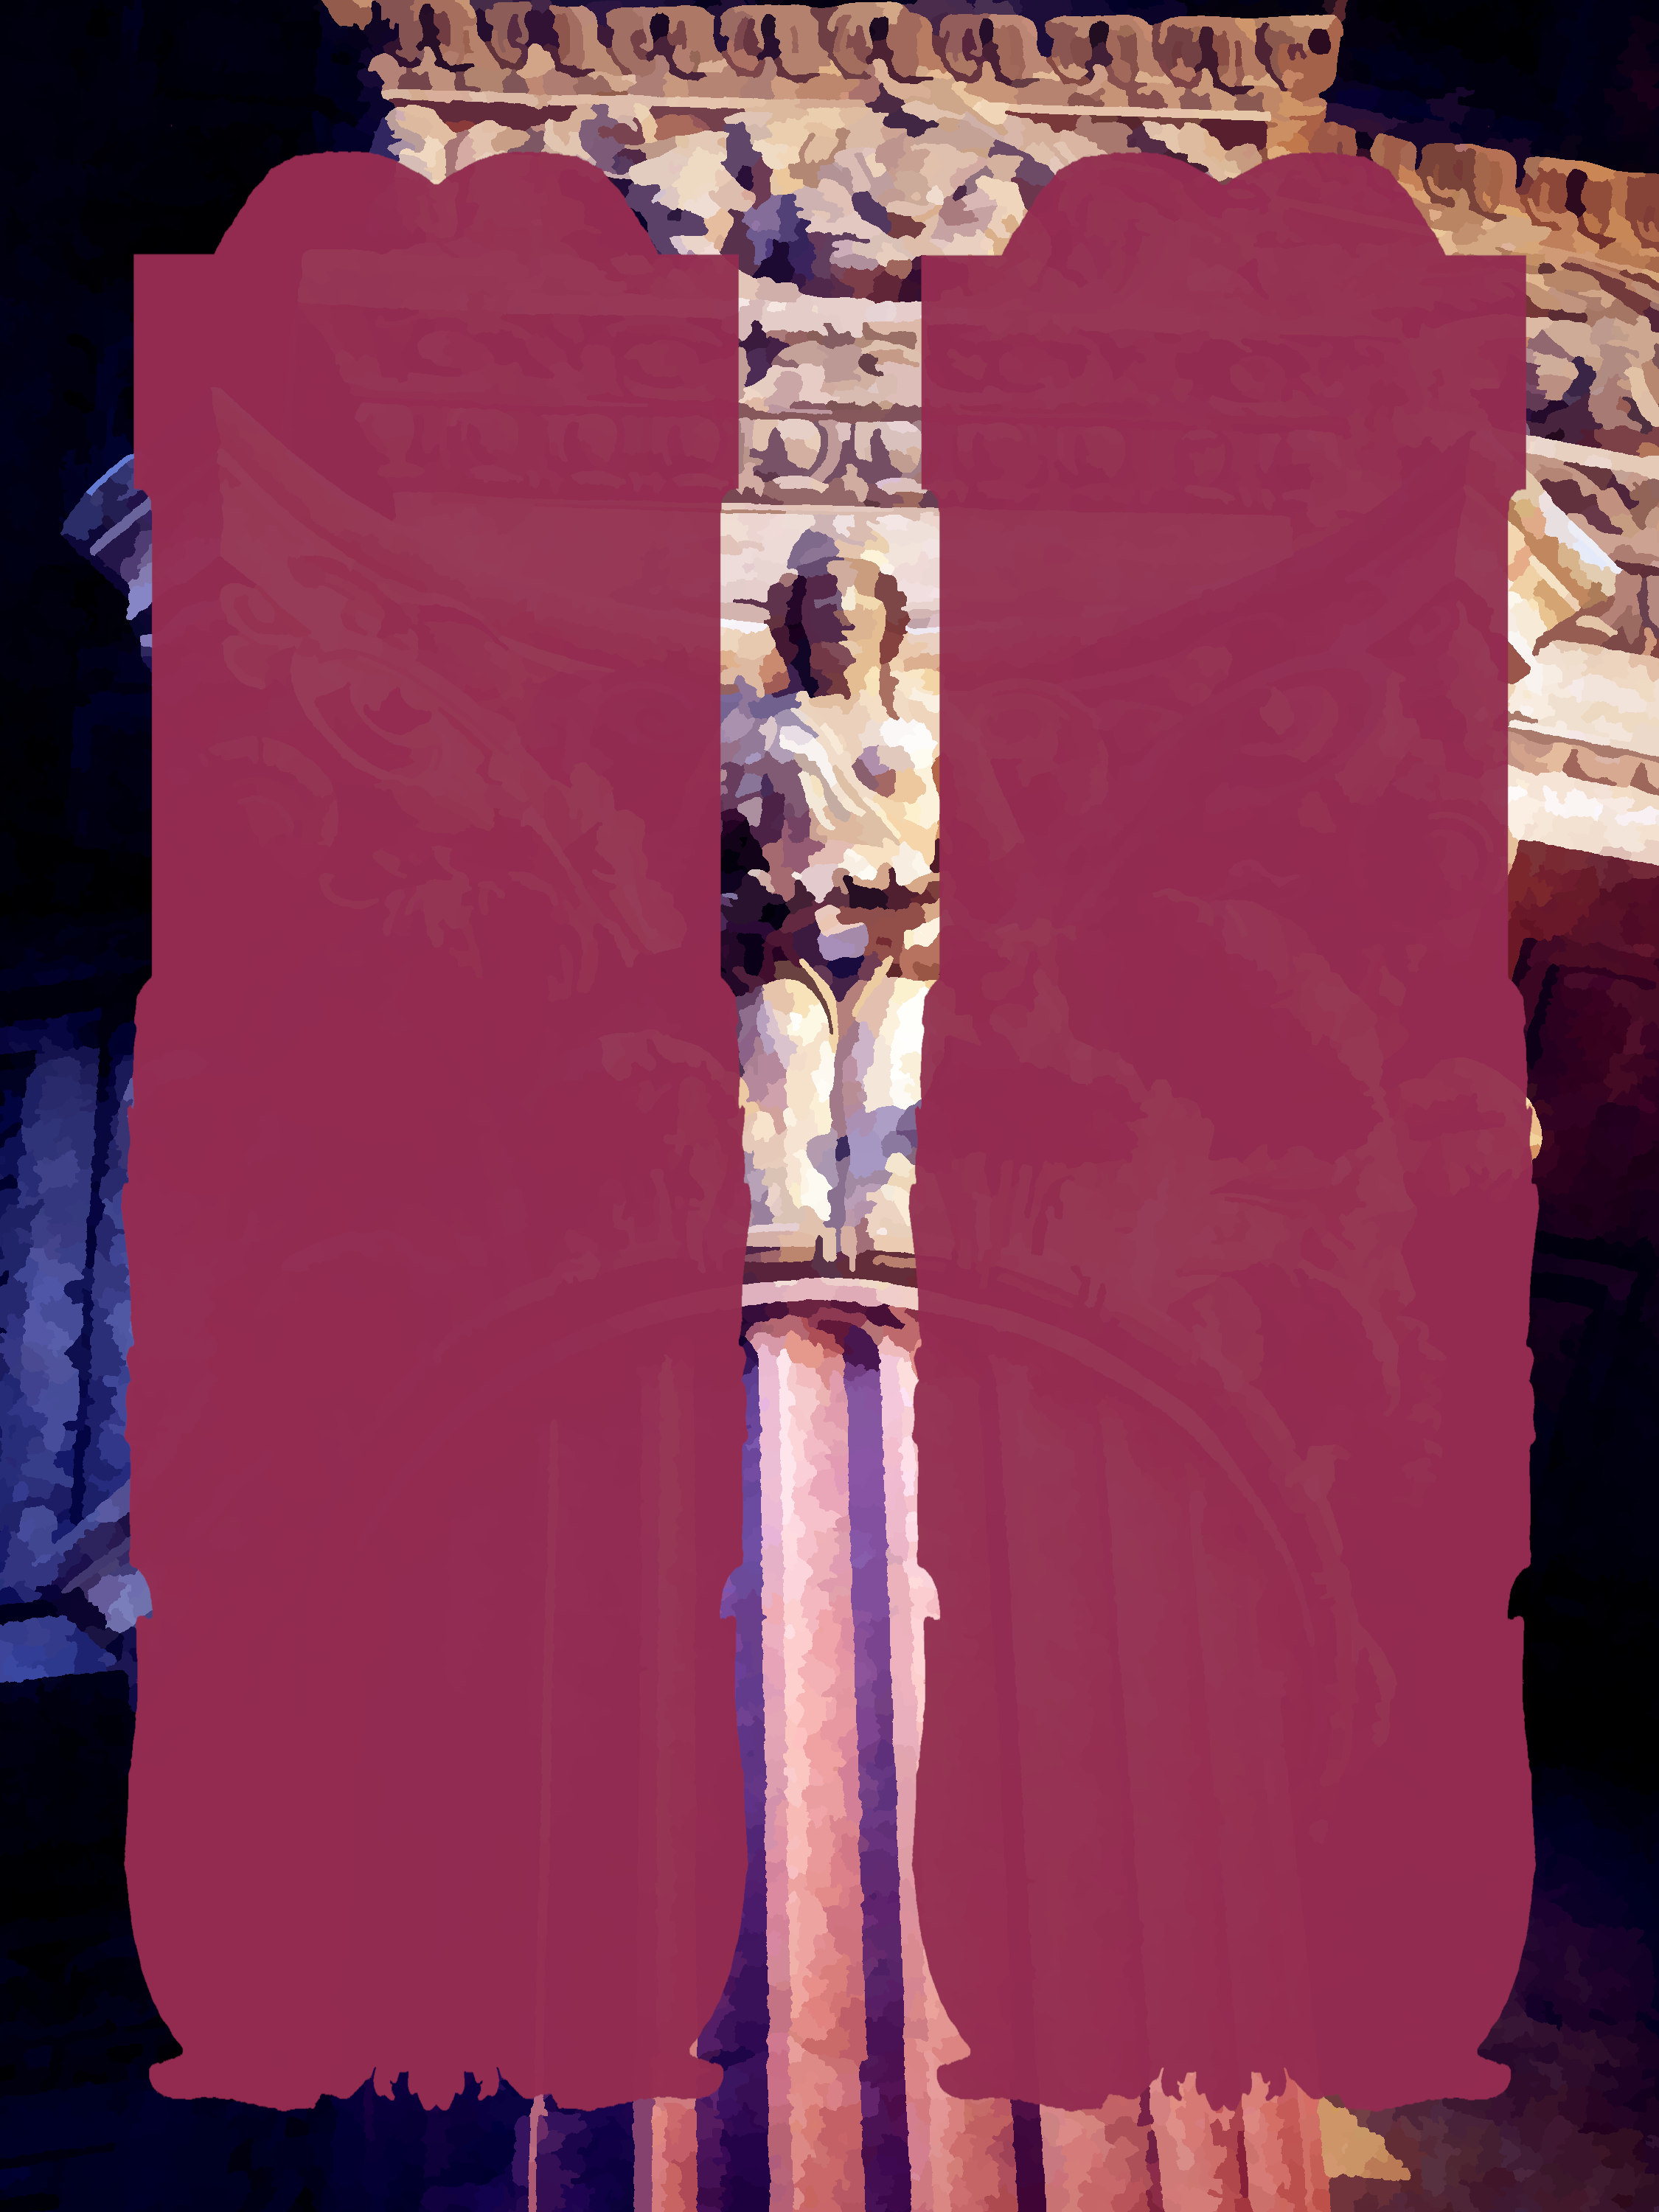
\includegraphics[width=\paperwidth,height=\paperheight]{column.jpeg}}
\setlength{\parskip}{1mm plus1mm minus1mm}
\setcounter{tocdepth}{3}
\setcounter{secnumdepth}{3}
\section*{}
\begin{center}
Read February 25, 1802.
\end{center}
\paragraph{}
The concordance of a variety of facts seems to render it most indisputable, that certain stony and metalline substances have, at different periods, fallen on the earth. Whence their origin, or whence they came, is yet, in my judgment, involved in complete obscurity.

The accounts of these peculiar substances, in the early annals, even of the Royal Society, have unfortunately been blended with relations which we now consider as fabulous; and the more ancient histories of stones fallen from heaven, from Jupiter, or from the clouds, have evidently confounded such substances with what have been termed \emph{Ceraunia}, \emph{Bætilia}, \emph{Ombria}, \emph{Brontia}, \emph{etc.} names altogether inappropriate to substances fallen on our globe. Indeed some mislead, and others are inexpressive.

The term Ceraunia, by a misnomer, deduced from its supposed origin, seems, as well as Bætilia,\footnote{Mercarti, Metallotheca Vaticana. page 241.} to have been anciently used to denote many species of stones, which were polished and shaped into various forms, though mostly wedge-like or triangular, sometimes as instruments, sometimes as oracles, and sometimes as deities. The import of the names, Ombria, Brontia, \emph{etc.} seems subject to the same uncertainty.

In very early ages, it was believed, that stones did in reality fall, as it was said, from heaven, or from the gods; these, either from ignorance, or perhaps from superstitious views, were confounded with other stones, which, by their compact aggregation, were better calculated to be shaped into different instruments, and to which it was convenient to attach a species of mysterious veneration. In modern days, because explosion and report have generally accompanied the descent of such substances, the name of thunderbolt, or thunderstone, has ignorantly attached itself to them; and, because a variety of substances accidentally present, near buildings and trees struck with lightning, have, with the same ignorance, been collected as thunderbolts, the thunderbolt and the fallen metalline substance have been ranked in the same class of absurdity. Certainly, since the phenomena of lightning and electricity have been so well identified, the idea of a thunderbolt is ridiculous. But the existence of peculiar substances fallen on the earth, I cannot hesitate to assert; and, on the concordance of remote and authenticated facts, I shall rest the assertion.

Mr. King, the learned author of \emph{Remarks concerning Stones said to have fallen from the Clouds, in these Days, and in ancient Times}, has adduced quotations of the greatest antiquity, descriptive of the descent of fallen stones; and, could it be thought necessary to add antique testimonies to those instanced by so profound an antiquarian, the quotations of Mons. Falconet, in his papers upon Bætilia, inserted in the \emph{Histoire des Inscriptions et Belles-Lettres}\footnote{Tom. 6. p. 519. and Tom. 23. p. 228.}; the quotations in Zahn's \emph{Specula Physico-mathematica Historiana}\footnote{Fol. 1696. Vol. 1. p. 385. where a long enumeration of stones fallen from the sky is given.}; the \emph{Fisica Sotterranea} of Giacinto Gemma; the works of Pliny, and others, might be referred to.

Dr. Chladni, in his \emph{Observations on the Mass of Iron found in Siberia, and on other Masses of the like Kind}, as well as in his \emph{Observations on Fire-balls and hard Bodies fallen from the Atmosphere}, has collected almost every modern instance of phenomena of this nature.

Mr. Southey relates an account, juridically authenticated, of a stone weighing 10 lbs. which was heard to fall in Portugal, Feb. 19, 1796, and was taken, still warm, from the ground.\footnote{Letters written during a short residence in Spain and Portugal. Page 239.}

The first of these peculiar substances with which chemistry has interfered, was the stone presented by the Abbé Bachelay to the Royal French Academy. It was found on the $13^{th}$ of September, 1768, yet hot, by persons who saw it fall. It is described as follows:

``La substance de cette pierre est d'un gris cendré pâle ; lorsqu'on en regarde le grain à la loupe, on apperçoit que cette pierre est parsemée d'une infinité de petits points brillans métalliques, d'un jaune pâle ; sa surface extérieure, celle qui, suivant M. l'Abbé Bachelay, n'étoit point engagée dans la terre, étoit couverte d'une petite couche trés-mince d'une matière noire, boursoufflée dans des endroits, et qui paroissoit avoir été fondue. Cette pierre, frappée dans l'intérieur avec l'acier, ne donnoit aucune étincelle ; si on frappoit, au contraire, sur la petite couche extérieure, qui paroissoit avoir été attaquée par le feu, on parvenoit à en tirer quelques-unes.''

The specific gravity of this stone was as 3535 to 1000.

The academicians analysed the stone, and found it to contain,
\begin{table}[H]
    \centering\bfseries
    \begin{tabular}{l r}
        Sulphur & $8\frac{1}{2}$ \\ 
        Iron & 36 \\
        Vitrifiable earth & $55\frac{1}{2}$ \\ \hline
        ~ & 100. \\
    \end{tabular}
\end{table}
\paragraph{}
Of their mode of analysis, I shall have occasion to speak hereafter. They were induced to conclude, that the stone, presented to the Academy by the Abbé Bachelay, did not owe its origin to thunder; that it did not fall from heaven; that it was not formed by mineral substances, fused by lightning; and that it was nothing but a species of pyrites, without peculiarity, except as to the hepatic smell disengaged from it by marine acid. ``Que cette pierre, qui peut-étre étoit couverte d'une petite couche de terre ou de gazon, aura été frappée par la foudre, et qu'elle aura été ainsi mise en évidence : la chaleur aura été assez grande pour fondre la superficie de la partie frappée, mais elle n'aura pas été assez long-tems continuée pour pouvoir pénétrer dans l'intérieur ; c'est ce qui fait que la pierre n'a point été décomposée. La quantité de matières métalliques qu'elle contenoit, en opposant moins de résistance qu'un autre corps au courant de matière électrique, aura peut-être pu contribuer même a déterminer la direction de la foudre.''

The Memoir is however concluded, by observing it to be sufficiently singular, that M. Morand le Fils had presented a fragment of a stone, from the environs of Coutances, also said to have fallen from heaven, which only differed from that of the Abbé Bachelay, because it did not exhale the hepatic smell with spirit of salt. Yet the academicians did not think any conclusion could be drawn from this resemblance, unless that the lightning had fallen by preference on pyritical matter.\footnote{See \emph{Journal de Physique}. Tom. 2. page 251.}

Mons. Barthold, Professeur à l'Ecole centrale du Haut-Rhin, gave I believe the next, and last,\footnote{A very interesting detail of a meteor, and of stones fallen in July, 1790, was given by Professor Baudin, in the \emph{Magazin für das Neueste aus der Physik}, by Professor Voigt.} analytical account of what he also denominates \emph{Pierre de Tonnerre}. He describes it thus: ``La masse de pierre connue sous le nom de Pierre de Tonnerre d'Ensisheim, pesant environ deux quintaux, a la forme extérieure arrondie, presque ovale, raboteuse, d'un aspect terne et terreux.''

``Le fond de la pierre est d'une couleur grise bleuâtre, parsemée de cristaux de pyrites, isolés, d'une cristalisation confuse, en quelques endroits écailleuses, ramassés, formant des nœuds et des petites veines, qui le parcourent en tout sens : la couleur des pyrites est dorée ; le poli leur donne un éclat d'acier, et, exposées à l'atmosphère, elles ternissent et brunissent. On distingue de plus, à l'œil nud, de la mine de fer grise, écailleuse, non sulfureuse, attirable à l'aimant, dissoluble dans les acides, peu oxidé, ou s'approchant beaucoup de l'état métallique.''

``La cassure est irrégulière, grenue, d'un grain un peu serré : dans l'intérieur on voit de très petites fentes. Elle ne fait pas feu au briquet ; sa contexture est si lâche qu'elle se laisse entamer au couteau. En la pilant, elle se réduit assez facilement en une poudre grise bleuâtre, d'une odeur terreuse. Quelquefois il se trouve des petits cristaux de mine de fer, qui résistent plus aux coups du pilon.''

The specific gravity of the piece in Professor Barthold's possession, was 3233, distilled water being taken at 1000.

The analysis of Mons. Barthold, of which I shall also have occasion to speak hereafter, gave in the 100,
\begin{table}[H]
    \centering\bfseries
    \begin{tabular}{l r}
        Sulphur & 2 \\
        Iron & 20 \\ 
        Magnesia & 14 \\ 
        Alumina & 17 \\ 
        Lime & 2 \\ 
        Silica & 42 \\ \hline
        ~ & 97. \\ 
    \end{tabular}
\end{table}
\paragraph{}
From the external characters, and from his analysis, the Professor considers the stone of Ensisheim to be argillo-ferruginous; and is of opinion that ignorance and superstition have attributed to it a miraculous existence, at variance with the first notions of natural philosophy.\footnote{See \emph{Journal de Physique. Ventose, An 8.} p. 169.}

The account next in succession is already printed in the Transactions of the Royal Society; but cannot be omitted, as it immediately relates to one of the substances I have examined. I allude to the letter received by Sir William Hamilton, from the Earl of Bristol, dated from Sienna, July $12^{th}$, 1794. ``In the midst of a most violent thunder-storm, about a dozen stones, of various weights and dimensions, fell at the feet of different persons, men, women, and children. The stones are of a quality not found in any part of the Siennese territory; they fell about eighteen hours after the enormous eruption of Mount Vesuvius; which circumstance leaves a choice of difficulties in the solution of this extraordinary phenomenon. Either these stones have been generated in this igneous mass of clouds, which produced such unusual thunder; or, which is equally incredible, they were thrown from Vesuvius, at a distance of at least 250 miles; judge then of its parabola. The philosophers here incline to the first solution. I wish much, Sir, to know your sentiments. My first objection was to the fact itself; but of this there are so many eyewitnesses, it seems impossible to withstand their evidence.'' (Phil. Trans. for 1795. p. 103.) Sir William Hamilton, it seems, also received a piece of one of the largest stones, which weighed upwards of five pounds; and had seen another, which weighed about one. He likewise observed, that the outside of every stone which had been found, and had been ascertained to have fallen from the clouds near Sienna, was evidently freshly vitrified, and was black, having every sign of having passed through an extreme heat; the inside was of a light grey colour, mixed with black spots and some shining particles, which the learned there had decided to be pyrites.

In 1796, a stone weighing 56 lbs. was exhibited in London, with several attestations of persons who, on the $13^{th}$ of December, 1795, saw it fall, near Wold Cottage, in Yorkshire, at about three o'clock in the afternoon. It had penetrated through 12 inches of soil and 6 inches of solid chalk rock; and, in burying itself, had thrown up an immense quantity of earth, toa great distance: as it fell, a number of explosions were heard, about as loud as pistols. In the adjacent villages, the sounds heard were taken for guns at sea; but, at two adjoining villages, were so distinct of something singular passing through the air, towards the habitation of Mr. Topham, that five or six people came up, to see if anything extraordinary had happened to his house or grounds. When the stone was extracted, it was warm, smoked, and smelt very strongly of sulphur. Its course, as far as could be collected from different accounts, was from the south-west. The day was mild and hazy, a sort of weather very frequent in the Wold hills, when there are no winds or storms; but there was not any thunder or lightning the whole day. No such stone is known in the country. There was no eruption in the earth; and, from its form, it could not come from any building; and, as the day was not tempestuous, it did not seem probable that it could have been forced from any rocks, the nearest of which are those of Hamborough Head, at a distance of twelve miles.\footnote{Extracted from the printed paper delivered at the place of exhibition.} The nearest volcano, I believe to be Hecla, in Iceland.

The exhibition of this stone, as a sort of show, did not tend to accredit the account of its descent, delivered in a handbill at the place of exhibition; much less could it contribute to remove the objections made to the fall of the stones presented to the Royal French Academy. But the Right Hon. President of the Royal Society, ever alive to the interest and promotion of science, observing the stone so exhibited to resemble a stone sent to him as one of those fallen at Sienna, could not be misled by prejudice: he obtained a piece of this extraordinary mass, and collected many references to descriptions of similar phenomena. At length, in 1799, an account of stones fallen in the East Indies was sent to the President, by John Lloyd Williams, Esq. which, by its unquestionable authenticity, and by the striking resemblance it bears to other accounts of fallen stones, must remove all prejudice. Mr. Williams has since drawn up the following more detailed narrative of facts.
\begin{center}
\emph{Account of the Explosion of a Meteor, near Benares, in the East Indies; and of the falling of some Stones at the same Time, about 14 Miles from that City.}
\end{center}
\begin{center}
By John Lloyd Williams, \emph{Esq. FRS.}
\end{center}
\paragraph{}
A circumstance of so extraordinary a nature as the fall of stones from the heavens, could not fail to excite the wonder, and attract the attention, of every inquisitive mind.

Among a superstitious people, any preternatural appearance is viewed with silent awe and reverence; attributing the causes to the will of the Supreme Being, they do not presume to judge the means by which they were produced, nor the purposes for which they were ordered; and we are naturally led to suspect the influence of prejudice and superstition, in their descriptions of such phenomena; my inquiries were therefore chiefly directed to the Europeans, who were but thinly dispersed about that part of the country.

The information I obtained was, that on the $19^{th}$ of December, 1798, about eight o'clock in the evening, a very luminous meteor was observed in the heavens, by the inhabitants of Benares and the parts adjacent, in the form of a large ball of fire; that it was accompanied by a loud noise, resembling thunder; and that a number of stones were said to have fallen from it, near Krakhut, a village on the north side of the river Goomty, about 14 miles from the city of Benares.

The meteor appeared in the western part of the hemisphere, and was but a short time visible: it was observed by several Europeans, as well as natives, in different parts of the country.

In the neighbourhood of Juanpoor, about 12 miles from the spot where the stones are said to have fallen, it was very distinctly observed by several European gentlemen and ladies; who described it as a large ball of fire, accompanied with a loud rumbling noise, not unlike an ill discharged platoon of musquetry. It was also seen, and the noise heard, by various persons at Benares. Mr. Davis observed the light come into the room where he was, through a glass window, so strongly as to project shadows, from the bars between the panes, on a dark coloured carpet, very distinctly; and it appeared to him as luminous as the brightest moonlight.

When an account of the fall of the stones reached Benares, Mr. Davis, the judge and magistrate of the district, sent an intelligent person to make inquiry on the spot. When the person arrived at the village near which the stones were said to have fallen, the natives, in answer to his inquiries, told him, that they had either broken to pieces, or given away to the Tesseldar (native collector) and others, all that they had picked up; but that he might easily find some in the adjacent fields, where they would be readily discovered, (the crops being then not above two or three inches above the ground,) by observing where the earth appeared recently turned up. Following these directions, he found four, which he brought to Mr. Davis: most of these, the force of the fall had buried, according to a measure he produced, about six inches deep, in fields which seemed to have been recently watered; and it appeared, from the man's description, that they must have lain at the distance of about a hundred yards from each other.

What he further learnt from the inhabitants of the village, concerning the phenomenon, was, that about eight o'clock in the evening, when retired to their habitations, they observed a very bright light, proceeding as from the sky, accompanied with a loud clap of thunder, which was immediately followed by the noise of heavy bodies falling in the vicinity. Uncertain whether some of their deities might not have been concerned in this occurrence, they did not venture out to inquire into it until the next morning; when the first circumstance which attracted their attention was, the appearance of the earth being turned up in different parts of their fields, as before mentioned, where, on examining, they found the stones.

The assistant to the collector of the district, Mr. Erskine, a very intelligent young gentleman, on seeing one of the stones, brought to him by the native superintendent of the collections, was also induced to send a person to that part of the country, to make inquiry; who returned with several of the stones, and brought an account similar to that given by the person sent by Mr. Davis, together with a confirmation of it from the Cauzy, (who had been directed to make the inquiry,) under his hand and seal.

Mr. Maclane, a gentleman who resided very near the village of Krakhut, gave me part of a stone that had been brought to him the morning after the appearance of the phenomenon, by the watchman who was on duty at his house; this, he said, had fallen through the top of his hut, which was close by, and buried itself several inches in the floor, which was of consolidated earth. The stone must, by his account, previous to its having been broken, have weighed upwards of two pounds.

At the time the meteor appeared, the sky was perfectly serene; not the smallest vestige of a cloud had been seen since the $11^{th}$ of the month, nor were any observed for many days after.

Of these stones, I have seen eight, nearly perfect, besides parts of several others, which had been broken by the possessors, to distribute among their friends. The form of the more perfect ones, appeared to be that of an irregular cube, rounded off at the edges; but the angles were to be observed on most of them. They were of various sizes, from about three to upwards of four inches in their largest diameter; one of them, measuring four inches and a quarter, weighed two pounds twelve ounces. In appearance, they were exactly similar: externally, they were covered with a hard black coat or incrustation, which in some parts had the appearance of varnish, or bitumen; and, on most of them were fractures, which, from their being covered with a matter similar to that of the coat, seemed to have been made in the fall, by the stones striking against each other, and to have passed through some medium, probably an intense heat, previous to their reaching the earth. Internally, they consisted of a number of small spherical bodies, of a slate colour, embedded in a whitish gritty substance, interspersed with bright shining spiculæ, of a metallic or pyritical nature. The spherical bodies were much harder than the rest of the stone: the white gritty part readily crumbled, on being rubbed with a hard body; and, on being broken, a quantity of it attached itself to the magnet, but more particularly the outside coat or crust, which appeared almost wholly attractable by it.

As two of the more perfect stones which I had obtained, as well as parts of some others, have been examined by several gentlemen well versed in mineralogy and chemistry, I shall not attempt any further description of their constituent parts; nor shall I offer any conjecture respecting the formation of such singular productions, or even record those which I have heard of others, but leave the world to draw their own inferences from the facts above related. I shall only observe, that it is well known there are no volcanos on the continent of India; and, as far as I can learn, no stones have been met with in the earth, in that part of the world, which bear the smallest resemblance to those above described.

\centerline{*\hspace{15mm}*\hspace{15mm}*\hspace{15mm}*\hspace{15mm}*}
\bigskip

It remains for me to speak of a substance mentioned in the \emph{Lithophylacium Bornianum}, Part 1. page 125, described thus: ``Ferrum retractorium, granulis nitentibus, matrice virescenti immixtis, (\emph{Ferrum virens} Linn.) cujus fragmenta, ab unius ad vigenti usque librarum pondus, cortice nigro scoriaceo circumdata, ad Plann, prope Tabor, circuli Bechinensis Bohemiæ, passim reperiuntur.''

The iron thus described, is moreover made remarkable by a note,\footnote{Quæ (fragmenta) 3 Julii, anni 1753, inter tonitrua, e cœlo pluisse creduliores quidam asserunt.} which observes, that credulous people assert it to have fallen from heaven, during a thunderstorm, on the $3^{rd}$ of July, 1753.

The collection of Baron Born, it is well known, has a place in the cabinet of the Right Hon. Charles Greville, who, from the effect produced by comparing the histories and structure of the Italian and Yorkshire stones with the description of this iron, was induced to search the collection of Born, where he discovered the very substance asserted to have fallen on the $3^{rd}$ of July, 1753. How far these four substances have resemblance to each other, it will soon appear not to be my province to anticipate.

The President having done me the honour to submit his specimens of the Yorkshire and Italian stones to my examination, I became indebted to Mr. Greville and Mr. Williams for a similar distinction: and, being thus possessed of four substances, to all of which the same origin had been attributed, the necessity of describing them mineralogically did not fail to present itself. To execute this task, no one could be more eager, and certainly no one better qualified, than the Count de Bournon. He has very obligingly favoured me with the following descriptions.
\begin{center}
\emph{Mineralogical Description of the various Stones said to have fallen upon the Earth.}
\end{center}
\begin{center}
By the Count de Bournon, \emph{FRS.}
\end{center}
\paragraph{}
The stones I am about to describe, are not of any regular shape; and those which were found in an entire state, that is, those which had not been broken, either by their fall or otherwise, were entirely covered with a black crust, the thickness of which was very inconsiderable.

The stones which fell at Benares, are those of which the mineralogical characters are the most striking: I shall therefore begin the following description with them; and shall afterwards make use of them, as objects of comparison, in describing the others.
\begin{center}
Stones from Benares.
\end{center}
\paragraph{}
These stones, as well as the others described in this Paper, whatever may be their size, are covered over the whole extent of their surface, with a thin crust, of a deep black colour: they have not the smallest gloss; and their surface is sprinkled over with small asperities, which cause it to feel, in some measure, like shagreen, or fish skin.

When these stones are broken, so as to show their internal appearance, they are found to be of a greyish ash colour; and of a granulated texture, very similar to that of a coarse gritstone: they appear evidently to be composed of four different substances, which may be easily distinguished, by making use of a lens.

One of these substances, which is in great abundance, appears in the form of small bodies, some of which are perfectly globular, others rather elongated or elliptical. They are of various sizes, from that of a small pin's head to that of a pea, or nearly so: some of them, however, but very few, are of a larger size. The colour of these small globules is grey, sometimes inclining very much to brown: and they are completely opaque. They may, with great ease, be broken in all directions: their fracture is conchoid, and shows a fine, smooth, compact grain, having a small degree of lustre, resembling in some measure that of enamel. Their hardness is such, that, being rubbed upon glass, they act upon it in a slight degree; this action is sufficient to take off its polish, but not to cut it: they give faint sparks, when struck with steel.

Another of these substances, is a martial pyrites, of an indeterminate form: its colour is a reddish yellow, slightly inclining to the colour of nickel, or to that of artificial pyrites. The texture of this substance is granulated, and not very strongly connected: when powdered, it is of a black colour. This pyrites is not attractable by the magnet; and is irregularly distributed through the substance of the stone.

The third of these substances consists in small particles of iron, in a perfectly metallic state, so that they may easily be flattened or extended, by means of a hammer. These particles give to the whole mass of the stone, the property of being attractable by the magnet; they are, however, in less proportion than those of pyrites just mentioned. When a piece of the stone was powdered, and the particles of iron separated from it, as accurately as possible, by means of a magnet, they appeared to compose about $\frac{2}{100}$ of the whole weight of the stone.

The three substances just described, are united together by means of a fourth, which is nearly of an earthy consistence. For this reason, it is easy to separate, with the point of a knife, or even with the nail, the little globular bodies above mentioned, or any other of the constituent parts of the stone we may wish to obtain. Indeed the stone itself may readily be broken, merely by the action of the fingers. The colour of this fourth substance, which serves as a kind of cement to unite the others, is a whitish grey.

The black crust with which the surface of the stone is coated, although it is of no great thickness, emits bright sparks, when struck with steel: it may be broken by a stroke with a hammer; and seems to possess the same properties as the very attractable black oxide of iron. This crust is, however, like the substance of the stone, here and there mixed with small particles of iron in the metallic state: they may easily be made visible, by passing a file over the crust, as they then become evident, on account of their metallic lustre. This is more particularly the case with respect to the crust of those stones which remain to be mentioned, they being much more rich in iron than that I have just described; a circumstance I think it needless to repeat, in the following descriptions of them. The stone now treated of, does not, when breathed upon, emit an argillaceous smell: the same remark may be applied to all the others.

The specific gravity of this stone is 3352.
\begin{center}
Stone from Yorkshire.
\end{center}
\paragraph{}
This stone, the constituent parts of which are exactly the same as those of the stones from Benares, differs from them, however,

First. In having a finer grain.

Secondly. That the substance described as being in the form of small globular or elliptical bodies, is not so constantly in those forms, but is also found in particles of an irregular shape; a circumstance that is not met with in the other stones: these bodies are likewise, in general, of a smaller size.

Thirdly. The proportion of martial pyrites, which has precisely the same characters as that in the stones from Benares, is less; on the contrary, that of the iron in a metallic state, is much greater. The quantity I was able to separate by means of the magnet, appeared to me to compose about eight or nine parts, in one hundred, of the weight of the whole mass. I observed many pieces of this iron, of a pretty considerable size; one of them, taken from a portion of the stone I had powdered, in order to separate the iron, weighed several grains.

The part of the stone which is in an earthy state, and which serves to connect the other parts together, has rather more consistence than that of the preceding stones; and its appearance does not differ much from that of decomposed felspar or kaolin. The stone itself, therefore, although by no means hard, is rather more difficult to break with the fingers.

The specific gravity of this stone is 3508.
\begin{center}
Stone from Italy.
\end{center}
\paragraph{}
This stone was in a perfectly entire state; consequently, its whole surface was covered over with the black crust peculiar to all stones of this kind. As the stone was of a very small size, it became necessary to sacrifice the whole of it to the investigation of its nature. Its grain was coarse, similar to that of the stones from Benares: in it might be perceived the same grey globular bodies, the same kind of martial pyrites, and the same particles of iron in the metallic state. The proportion of these last was much less than in the stone from Yorkshire; but rather greater than in the stones from Benares. The same kind of grey earthy substance served to connect the different parts together; and nothing more could be perceived, except a few globules, which consisted wholly of black oxide of iron, attractable by the magnet, and one single globule of another substance, which appeared to differ from all those we have already described. This last substance had a perfectly vitreous lustre, and was completely transparent: it was of a pale-yellow colour, slightly inclining to green; and its hardness was rather inferior to that of calcareous spar. The quantity of it, however, was too small to be submitted to such an investigation as might have determined its nature. The black crust which covered the stone, was rather thinner than that of the stones already described; and seemed to have undergone a kind of contraction, which had produced in it a number of fissures or furrows, thereby tracing upon the surface the appearance of compartments, similar in some measure to what is observed in the stones called Septaria.

The specific gravity of this stone was 3418.
\begin{center}
Stone from Bohemia.
\end{center}
\paragraph{}
The internal structure of this stone is very similar to that of the stone from Yorkshire. Its grain is finer than that of the stones from Benares: in it may be observed the same grey substance, both in small globules and in particles of an irregular shape; also the same particles of metallic iron. The same kind of earthy substance likewise served to connect the other parts together.

This stone, however, differs materially from the others.

First. The particles of pyrites cannot be seen without a lens.

Secondly. It contains a much larger quantity of iron in the metallic state; insomuch, that the proportion of that metal, separated from it by means of the magnet, amounted to about $\frac{25}{100}$ of the weight of the whole.

This stone has also (owing perhaps to its having remained a much longer time in the earth than the preceding ones, all of which were taken up nearly at the very instant of their fall,) another difference, \emph{viz.} many of the particles of iron in a metallic state, have undergone an oxidizement at their surface; a circumstance that has produced a great number of spots, of a yellowish brown colour, and very near to each other, over a part of its internal substance. This oxidizement, by adding to the bulk, and to the force of action, of the part we have described as serving by way of cement to the other constituent parts of the stone, has occasioned a greater degree of adhesion between these parts, and has rendered the substance of the stone more compact.

The great quantity of iron in a metallic state which this stone contains, added to its greater compactness, makes it capable of receiving a slight degree of polish; whereas it is impossible to give any polish to the others. When polished, the iron becomes very evident, in the polished part; appearing in the form of small specks, almost close to each other, which have the colour and lustre peculiar to that metal: these specks are, in general, nearly of an equal size.

The black crust of this stone is similar to that of the others.

The specific gravity of the stone is 4281.

It is easy to perceive, from the foregoing description, that these stones, although they have not the smallest analogy with any of the mineral substances already known, either of a volcanic or any other nature, have a very peculiar and striking analogy with each other. This circumstance renders them truly worthy to engage the attention of philosophers; and naturally excites a desire of knowing to what causes they owe their existence.

\centerline{*\hspace{15mm}*\hspace{15mm}*\hspace{15mm}*\hspace{15mm}*}
\bigskip

I proceed to consider the assistance to be derived from chemistry, in distinguishing these stones from all other known substances, and in establishing the assertion, that they have fallen on the earth.

The analysis made by the French Academicians, of the stone presented to them by the Abbé Bachelay, was, in part, conducted by the ever to be deplored Lavoisier; but it was performed before that celebrated author had enriched chemistry with his last discoveries, and before he had given birth to the system under which it flourishes. The result of this analysis might well induce the conclusion, that the subject of it was common pyritical matter. It was unfortunately made of an aggregate portion of the stone, and not of each distinct substance, irregularly disseminated through it. The proportions obtained were, consequently, as accidental as the arrangement of every substance in the mass.

The analysis of M. Barthold, of the stone of Ensisheim, is subject to the same objections: but, after having the advantage of the foregoing descriptions, the researches which follow cannot be supposed altogether liable to a similar fatality.
\begin{center}
Examination of the Stone from Benares.
\end{center}
\paragraph{}
This stone, as the Count de Bournon has already remarked, has the most distinguished characters. Indeed it is the only one of the four, sufficiently perfect (if I be allowed that expression) to be subjected to anything approaching to a regular analysis.

The crust, or external black covering, is the first substance to which the attention is naturally directed. When a portion of this crust had been detached with a knife, or a file, and finely pulverized, I separated the particles attractable by a magnet; and digested the unattractable portion with nitric acid, which was presently decomposed; but, owing to a strong adherence of some of the interior and earthy parts of the stone, it did not disentangle the coating or metalline part without some difficulty. The acid being sufficiently neutralized, the solution was passed through a filter, and saturated to excess with ammonia. An abundant precipitate of oxide of iron was produced; and, when this oxide was separated, I observed the saline liquor to have a greenish colour. I evaporated it to dryness; and redissolved the dry salt in distilled water. No precipitate was formed during the evaporation, nor was the colour of the solution entirely destroyed. It appeared to me like a triple salt, described by Mr. Hermstadt\footnote{\emph{Annales de Chimie}. Tom. 22. p. 108.} as an ammoniacal nitrate of nickel. By examination with prussiate of ammonia, it yielded a whitish precipitate, inclining to a violet colour; and, by various properties, I was soon confirmed in the opinion, that nickel was present. Since I shall have occasion more than once to treat of the triple compound, and since it has been only mentioned by Mr. Hermstadt, it is necessary now to detail some of its distinctive characters. The same chemist informs us, that the three mineral acids, with ammonia, enter into similar combinations with nickel; and I have observed, that oxide of nickel can be dissolved by nitrate and muriate of ammonia. The muriate seems to take up the largest quantity. The colour of this salt is by no means uniform: it is sometimes grass green, violet, rose colour, inclining to purple, and I have seen it almost colourless. It seems to be purple, and to incline to rose colour and violet, when all the oxide of nickel is not united to both acid and alkali, but, from the deficiency of salt, is held in solution by an excess of ammonia. In this case, evaporation, of course, precipitates the nickel in the state of oxide, which is of a whitish green colour.

The nickel cannot be \emph{precipitated} from a perfectly formed triple salt, by any reagent I have tried, except by a prussiate, or a hydrogenized sulphuret of ammonia. Potash and lime, as well as, I presume, other bodies, standing in the order of affinities before ammonia, decompose the salt; but the nickel is then continued in solution by the disengaged ammonia.

As it may be imagined that I have occasionally met with copper, when I describe a violet or purple ammoniacal solution, it is right to observe, that to avoid this error, I have either reduced the liquor to a neutral state, and endeavoured, without success, to obtain from it a precipitate, with a solution of sulphureted hydrogen gas; or, by adding an acid to slight excess, and immersing a piece of iron, I have not been able to detect a trace of copper. These, and many other trials, when they do not appear to be made before the estimation of the quantities of nickel, have been constantly made afterwards.

But, to return to the incrustation or coating of the stone, the decomposition of the nitric acid showed the presence of matter at least nearly metallic, although not attractable; and the examinations made of the liquor, from which the iron was precipitated, ascertained the presence of nickel beyond dispute. The difficulty of obtaining the coating of the stone, either distinct from matter not belonging to it, or in sufficient quantity, induced me to relinquish the idea of attempting to give the proportions of its constituent parts.

The stone being deprived of its covering, the shining particles irregularly disseminated, next demand examination. I first examined the pyrites. Their very loose texture made it exceedingly difficult to collect the weight of 16 grains, which was however effected by the dexterity of the Count de Bournon.

I digested these, at a low heat, with weak muriatic acid; which acted gradually, and disengaged a trifling but sensible quantity of sulphureted hydrogen gas. After several hours, I found the acid discontinued its action. The whole metalline part appeared in solution; but sulphur and earthy particles were observable. The sulphur, from its small specific gravity, was suspended through the solution; whilst the earthy matter, which could not be separated by mechanical means, was fortunately left at the bottom of the digesting vessel. I decanted off the solution, holding suspended the sulphur; and, by repeated washing, separated everything belonging to the pyrites from the insoluble earthy matter, the subtraction of which reduced the weight of real pyrites to 14 grains. I next obtained the sulphur, by filtration. When it was as dry as I could make it, without fear of its being sublimed, its weight was two grains. To the filtrated liquor I added nitrate of barytes, by way of detecting any sulphuric acid which might have been present; but no cloudiness ensued. I then separated, by sulphate of ammonia, the barytes thus added, and precipitated the iron with ammonia. The liquor, on the subsidence of oxide of iron, appeared of a violet purple colour: it contained nickel, which I threw down with sulphureted hydrogen gas, there being already a sufficient excess of ammonia in the saline liquor to form an alkaline hydrogenized sulphuret. The oxide of iron, after ignition, weighed 15 grains; and the sulphuret of nickel, reduced to an oxide, weighed, after the same treatment, something more than one grain. The proportions of the substances contained in the pyrites of the stone from Benares, may therefore be considered nearly thus:
\begin{table}[H]
    \centering\bfseries
    \begin{tabular}{l r}
        Sulphur & 2 Grains.  \\
        Iron & $10\frac{1}{2}$ Grains. \\
    \end{tabular}
\end{table}
\paragraph{}
Since 15 grains of the oxide represent about that quantity of iron,
\begin{table}[H]
    \centering\bfseries
    \begin{tabular}{l r}
        Nickel, nearly & 1 Grains.   \\
        Extraneous earthy matter & 2 Grains. \\ \hline
        ~ & $15\frac{1}{2}$ Grains. \\ 
    \end{tabular}
\end{table}
\paragraph{}
It is observable that, notwithstanding the loss appears to be only half a grain, it was probably more, because the sulphur could not be reduced to the same state of dryness in which it existed when in combination with the iron; not to say that it was, in a small degree, volatilized with the hydrogen gas disengaged during the solution.

The weight of nickel is a mere estimation. We are not yet sufficiently acquainted with that metal to speak of it with accuracy, except as to its presence. Upon the whole, however, it may be concluded, that these pyrites are of a very particular nature; for, although Henkel has observed that sulphur may be separated from pyrites by muriatic acid, it is by no means the usual habitude of pyrites to be of such easy decomposition.

The other shining particles immediately seen, when the internal structure of the stone is exposed, are the malleable iron. Before I state the examination of this iron, I must remark, that preliminary experiments having shown me it contained nickel, I treated several kinds of the most pure irons I could obtain, with nitric acid; and precipitated the oxide from the metallic salt by ammonia. The quantity of oxide I obtained from 100 grains of iron, was from 144 to 146. I may consequently infer, that 100 grains of pure iron acquires, by such a process, 45 grains of oxygen; and that, whenever a metallic substance, supposed to be iron, does not, under the same circumstances, acquire the same proportionate weight, something is either volatilized, or left in solution. Hence, when a metallic alloy of nickel and iron presents itself, a judgment may, at least, be formed of the quantity of nickel, by the deficiency of weight in the precipitated oxide of iron.

This mode of treatment was not allowed me in the examination of the coating of the stone, because it was impossible to know in what state of oxidizement the iron existed. But, as the particles disseminated through the whole mass, are clearly metallic, a very tolerable idea of the quantities of nickel contained in them will be obtained, by noting the quantity of oxide of iron separated, as above described. 25 grains of these metallic particles were therefore heated with a quantity of nitric acid, much more than sufficient to dissolve the whole. Some earthy matter, which, as in a former case, was not separable by mechanical means, remained after a complete solution of the metal had been effected. This earthy matter, after being ignited, weighed two grains. The real matter of the present examination, was therefore reduced to 23 grains, and was in complete solution. I added ammonia to a very sensible excess. The oxide of iron was thereby precipitated, and, being collected and ignited, it weighed 24 grains; whereas, according to my experiments, $33\frac{1}{2}$ grains should have been produced from the solution, had it contained nothing but iron. I examined the saline liquor, when free from ferruginous particles, and discovered it to be the triple salt of nickel. Hence, allowing for loss, the quantity of nickel may be estimated, by calculating the quantity of iron contained in 24 grains of oxide. Thus, if 145 grains of oxide contain 100 of iron, about $16\frac{1}{2}$ are contained in 24 of oxide. This would suppose the 23 grains of alloy to consist of $16\frac{1}{2}$ iron and $6\frac{1}{2}$ nickel; which, if the usual loss be added to the $16\frac{1}{2}$ grains of iron, and deducted from the nickel, may not be very remote from the truth.

I shall next examine the globular bodies, also irregularly dispersed throughout the stone. A number of them were reduced to fine powder; but nothing metallic could be separated by the magnet. As a preliminary experiment, I sought for pyrites, by digestion with muriatic acid; but no hepatic smell was in the least perceivable, nor was white carbonate of lead at all altered by being held over the mixture. I therefore conclude these globular bodies do not envelope either iron or pyrites. By way of analysis, I treated 100 grains with potash, in a silver crucible; and, after the usual application of a red heat, separated as much silica as possible, by muriatic acid and evaporation. The silica being collected on a filter, carbonate of potash was added to the filtrated liquor; by which, a precipitate, almost wholly ferruginous, was produced. This precipitate was collected in the common way; then boiled with potash, to extract alumina; and, by supersaturating the alkaline liquor with muriatic acid, and precipitating by carbonate of ammonia, an earth was gathered, which I afterwards found to be partly, if not entirely, siliceous. After redissolving, in muriatic acid, the portion of the ferruginous matter rejected by the potash, I precipitated by ammonia, what I took to be entirely oxide of iron; but, after igniting it, and again attempting to redissolve the whole in muriatic acid, more silica was left. The non-existence of lime was proved, by the addition of carbonate of ammonia, immediately after the same alkali, pure, had thrown down what I took wholly for oxide of iron. I had now obtained everything in the subject of my analysis, except magnesia and nickel. The former, and a trace of the latter, were held by carbonic acid in the liquor, from which the ferruginous precipitate was, in the first instance, thrown down by carbonate of potash; and the latter was found in the last-named muriate of ammonia. I disengaged the magnesia, by the assistance of potash, and by evaporating to dryness. The oxide of nickel was precipitated by hydrogenized sulphuret of ammonia.

Under all circumstances, I am induced to state the proportions of constituent parts thus:
\begin{table}[H]
    \centering\bfseries
    \begin{tabular}{l r}
        Silica & 50 \\ 
        Magnesia & 15 \\ 
        Oxide of iron & 34 \\ 
        Oxide of nickel & $2\frac{1}{2}$   \\ \hline
        ~ & $101\frac{1}{2}$. \\
    \end{tabular}
\end{table}
\paragraph{}
The excess of weight, instead of the usual loss, is owing to the difference of oxidizement of the iron, in the stone and in the result of the analysis; which will be found to be the case in all analyses of these substances; indeed it is always necessary to reduce the oxide to the red state, as being the only one to be depended upon. To avoid future repetition, I shall also observe, first, that by preliminary experiments, I could not detect any other substance than those mentioned. Secondly, that the earth obtained as alumina, appeared to me to be mostly, if not entirely, siliceous; because, after it had been ignited, and again treated with potash and muriatic acid, I found it was very nearly all precipitated by evaporation. Thirdly, I examined, and judged of, the silica collected from the oxide of iron, in the same way. Fourthly, the weight of the magnesia is given, not immediately, as obtained by evaporation, but after a subsequent solution in an acid, and precipitation by potash. And, fifthly, the proportions are taken from the mean of two analyses.

Nothing remains to be examined, of the stone from Benares, except the earthy matter, forming a cement or matrix for the substances already examined. 100 grains of this matter were, by mechanical means, separated as perfectly as possible, from the pyrites, iron, and globular bodies, and analysed as above. The mean result of two analyses gave,
\begin{table}[H]
    \centering\bfseries
    \begin{tabular}{l r}
        Silica & 48 \\ 
        Magnesia & 18 \\ 
        Oxide of iron & 34 \\ 
        Oxide of nickel & $2\frac{1}{2}$   \\ \hline
        ~ & $102\frac{1}{2}$. \\
    \end{tabular}
\end{table}
\begin{center}
Examination of the Stone from Sienna.
\end{center}
\paragraph{}
The external coating of this stone appeared to have the same characters as that of the stone from Benares.

The pyrites, although certainly present, were not crystallized in such groups as in the preceding stone; nor could they be separated by mechanical means.

The attractable metal was easily separated by the magnet; but $8\frac{1}{2}$ grains only were collected. I treated them with nitric acid and ammonia, as in a preceding case. Nearly one grain of earthy matter was insoluble; the weight was therefore reduced to rather less than 8 grains. The oxide of iron, precipitated by ammonia, weighed 8 grains; and the saline liquor gave abundant indications of nickel. As 8 grains of this oxide of iron contain nearly 6 of metal, the quantity of nickel, in the bare 8 grains, may be estimated between 1 and 2 grains. Some globular bodies were extracted, but too few to analyse.

Since the pyrites could not be separated, I collected 150 grains of the stone, freed from iron by the magnet, and as exempt as possible from globular bodies. These 150 grains, I first digested with muriatic acid, that the pyrites might be decomposed, and everything taken up which could be dissolved by that menstruum. A very decided disengagement of sulphureted hydrogen gas was occasioned. When the acid could produce no further action, I collected the undissolved matter on a filter, and boiled it with the most concentrate nitric acid, in hopes of being able to convert the sulphur, previously liberated, into sulphuric acid; but my endeavours were fruitless; for, upon the addition of nitrate of barytes to the nitric solution, rendered previously transparent, a very insignificant quantity of sulphate of barytes was obtained. The surplus of barytic nitrate was removed by sulphate of potash. I next completely edulcorated the mass which remained insoluble, after the action of the muriatic and nitric acids; and, adding the water of edulcoration to the muriatic and nitric liquors, evaporated the whole for silica. I then submitted the mass, undissolved by the acids and the water, to the treatment with potash, muriatic acid, and evaporation, which was, in the first instance, applied to the stone from Benares. The first precipitation was, as in that analysis, also effected with carbonate of potash; but, instead of endeavouring immediately to extract alumina, I ignited the precipitate, that the alumina or silica remaining might be rendered insoluble. After the ignition, I separated the oxide of iron with very concentrate muriatic acid; and the earths, which were left perfectly white, I heated with potash, until they were again capable of being taken up by the same acid. The solution so made, was slowly evaporated; and, as very nearly everything was deposited during the evaporation, I conclude all was silica. The proportions resulting from this single analysis, without the weight of sulphur contained in the pyrites irregularly disseminated through the whole, were,
\begin{table}[H]
    \centering\bfseries
    \begin{tabular}{l r}
        Silica & 70 \\
        Magnesia & 34 \\
        Oxide of iron & 52 \\
        Oxide of nickel & 3 \\ \hline
        ~ & 159. \\
    \end{tabular}
\end{table}
\begin{center}
Examination of the Stone from Yorkshire.
\end{center}
\paragraph{}
The mechanical separation of the substances in this stone being as difficult as in the preceding case, I was necessarily satisfied with submitting it to the same treatment. I collected, however, 34 grains of malleable particles; which, by the process already more than once mentioned, left 4 grains of earthy matter; and, by yielding $37\frac{1}{2}$ of oxide of iron, indicated about 4 grains of nickel.

150 grains of the earthy part of the stone were, by analysis, resolved into,
\begin{table}[H]
    \centering\bfseries
    \begin{tabular}{l r}
        Silica & 75 \\
        Magnesia & 37 \\
        Oxide of iron & 48 \\
        Oxide of nickel & 2 \\ \hline
        ~ & 162. \\
    \end{tabular}
\end{table}
\begin{center}
Examination of the Stone from Bohemia.
\end{center}
\paragraph{}
The probability of never being able to obtain another specimen of the very remarkable fragment of this substance, did not allow me to trespass more on the liberality of Mr. Greville, than to detach a small portion. I found it of similar composition to that of the three preceding stones; and the Count de Bournon has already shown the proportionate quantity of the attractable metal to be very considerable. $16\frac{1}{2}$ grains, left $2\frac{1}{2}$ of extraneous earthy matter; and yielded, by the treatment with nitric acid and ammonia, $17\frac{1}{2}$ grains of oxide of iron. This would seem to induce an estimation of $1\frac{1}{2}$ of nickel in 14 grains, or about 9 per cent.

55 grains of the earthy part of the stone, by the analytical treatment of the two former, afforded,
\begin{table}[H]
    \centering\bfseries
    \begin{tabular}{l r}
        Silica & 25 \\
        Magnesia & $9\frac{1}{2}$ \\
        Oxide of iron & $23\frac{1}{2}$ \\ 
        Oxide of nickel & $1\frac{1}{2}$ \\ \hline
        ~ & $59\frac{1}{2}$. \\
    \end{tabular}
\end{table}
\paragraph{}
The unusual increase of weight in the result of the three last analyses, notwithstanding the entire loss of the sulphur in the pyrites, is obviously owing to the metallic state of the iron combined with the sulphur, as was shown in a former instance.

I have now concluded the chemical examination of these four extraordinary substances. It unfortunately differs from the analysis made by the French Academicians, of the stone presented to them by the Abbé Bachelay, as well as from that made by Professor Barthold, of the stone of Ensisheim. It is at variance with that of the Academicians, inasmuch as they found neither magnesia nor nickel. It differs from that of Mr. Barthold, as he did not find nickel, but discovered some lime, with 17 per cent. of alumina. With regard to these differences, I have to submit to the chemical world, whether magnesia might not have eluded the action of an acid, when the aggregation of the integrant parts of the stone was not destroyed by treatment with potash. As to the existence of alumina, I do not absolutely deny it; yet I must observe, that the whole of the earth which seemed to have any resemblance, however small, to alumina, was at most 3 per cent. and there seems good reason to consider it as silica. Respecting the existence of lime in the stone of Ensisheim, I must appeal to Professor Barthold, whether, supposing lime a constituent part, sulphate of lime should not have been formed, as well as sulphate of magnesia, when sulphuric acid was generated by igniting the earths and pyrites. And, as to the proportion of alumina, in the same stone, I would ask, at least, whether it would have been so considerable, if the solutions formed by acids, after the treatment with potash, had been evaporated to the requisite dryness: not to observe, that no mention is made of any examination of the properties of the earth called alumina. In the proportion of magnesia, I have the satisfaction to find my analysis correspond very nearly with that of Professor Barthold; and, if what he considered alumina were supposed silica, the stone presented to the French Academy, the stone of Ensisheim, and the four I have examined, would agree very nearly in siliceous proportions. With respect to the nickel, I am confident it would have been found in all, had the metallic particles been separately examined. But, whatever be these variations, the mineralogical description of the French Academicians, of Mr. Barthold, and of the Count de Bournon, all exhibit a striking conformity of character, common to each of these stones; and I doubt not but the similarity of component parts, especially of the malleable alloy, together with the near approach of the constituent proportions of the earths contained in each of the four stones, the immediate subject of this Paper, will establish very strong evidence in favour of the assertion, that they have fallen on our globe. They have been found at places very remote from each other, and at periods also sufficiently distant. The mineralogists who have examined them, agree that they have no resemblance to mineral substances, properly so called; nor have they been described by mineralogical authors. I would further urge the authenticity of accounts of fallen stones, and the similarity of circumstances attendant on such phenomena; but, to the impartial it would be superfluous, and, to those who disbelieve whatever they cannot explain, it would be fruitless. Attempts to reconcile occurrences of this nature with known principles of philosophy, it is true, are already abundant; but (as the Earl of Bristol has well expressed) they leave us a choice of difficulties equally perplexing. It is however remarkable, that Dr. Chladni, who seems to have indulged in these speculations with most success, should have connected the descent of fallen stones with meteors; and that, in the narrative of Mr. Williams, the descent of the stones near Benares, should have been immediately accompanied with a meteor.

No luminous appearance having been perceived during the day on which the stone fell in Yorkshire, it must be admitted, rather militates against the idea, that these stones are the substances which produce or convey the light of a meteor, or that a meteor must necessarily accompany them.\footnote{In the account of the stone which fell in Portugal, no mention is made, either of a meteor or lightning.} Yet the stones from Sienna fell amidst what was imagined lightning, but what might in reality have been a meteor. Stones were also found, after the meteor seen in Gascony, in July, 1790. And Mr. Falconet, in the memoir I have already quoted, relates, that the stone which was adored as the mother of the gods, was a Bœtilia; and that it fell at the feet of the poet Pindar, enveloped in a ball of fire. He also observes, that all the Bœtilia had the same origin.

I ought not perhaps to suppress, that in endeavouring to form an artificial black coating on the interior surface of one of the stones from Benares, by sending over it the electrical charge of about 37 square feet of glass, it was observed to become luminous, in the dark, for nearly a quarter of an hour; and that the tract of the electrical fluid was rendered black. I by no means wish to lay any stress upon this circumstance; for I am well aware, that many substances become luminous by electricity.

But, should it ever be discovered that fallen stones are actually the bodies of meteors, it would not appear so problematical, that such masses as these stones are sometimes represented, do not penetrate further into the earth: for meteors move more in a horizontal than in a perpendicular direction; and we are as absolutely unacquainted with the force which impels the meteor, as with the origin of the fallen stone.

Before I close this subject, I may be particularly expected to notice the meteor which, a few months ago, traversed the county of Suffolk. It was said, that part of it fell near Saint Edmundsbury, and even that it set fire to a cottage in that vicinity. It appeared, from inquiries made on the spot, that something, seemingly from the meteor, was, with a degree of reason, believed to have fallen in the adjacent meadows; but the time of the combustion of the house did not correspond with the moment of the meteor's transition. A phenomenon much more worthy of attention, has since been described in the Philosophical Magazine. On the night of the $5^{th}$ of April, 1800, a body wholly luminous, was seen, in America, to move with prodigious velocity. Its apparent size was that of a large house, 70 feet long; and its elevation above the surface of the earth, about 200 yards. The light produced effects little short of sunbeams; and a considerable degree of heat was felt by those who saw it, but no electric sensation. Immediately after it disappeared in the north-west, a violent rushing noise was heard, as if the phenomenon were bearing down the forest before it; and, in a few seconds after, there was a tremendous crash, causing a very sensible earthquake. Search being afterwards made in the place where the burning body fell, every vegetable was found burnt, or greatly scorched, and a considerable portion of the surface of the earth broken up. We have to lament, that the authors of this account did not search deeper than the surface of the ground. Such an immense body, though moving in a horizontal direction, could not but be buried to a considerable depth. Should it have been more than the semblance of a body of a peculiar nature, the lapse of ages may perhaps effect what has now been neglected; and its magnitude and solitary situation become the astonishment of future philosophers.

This leads me to speak of the solitary mass of what has been called native iron, which was discovered in South America, and has been described by Don Rubin de Celis. Its weight was about 15 tons. The same author mentions another insulated mass of the same nature. The whole account is exceedingly interesting; but, being already published in the Philosophical Transactions for the year 1788, it needs not be here repeated.

Mr. Proust has shown the mass particularly described, not to be wholly iron, but a mixture of nickel and iron. The Trustees of the British Museum, who are in possession of some fragments of this mass, sent to the Royal Society by Don Rubin de Celis, have done me the honour to permit me to examine them; and I have great satisfaction in agreeing with a chemist so justly celebrated as Mr. Proust.

The connexion which naturally exists between one mass of native iron and another, immediately turns our attention to the native iron in Siberia, described by Pallas; and this, we are told, the Tartars considered as a sacred relic, which had dropped from heaven. The nickel found in the one mass, and the traditional history of the other, not to compare the globular bodies of the stone from Benares with the globular concavities and the earthy matter of the Siberian iron, tend to the formation of a chain between fallen stones and all kinds of native iron. How far any real affinity exists between these several substances, very obliging friends have afforded me an opportunity to form some judgment. I am indebted to Mr. Greville and Mr. Hatchett for portions of almost every known native iron: and the Count de Bournon has done me the favour particularly to describe them as follows.
\begin{center}
\emph{Description of various Kinds of native Iron.}
\end{center}
\begin{center}
By the Count de Bournon.
\end{center}
\paragraph{}
The great number of particles of iron, in a perfectly metallic state, contained in the stone from Bohemia, and the said particles being so near each other, naturally lead to some reflections respecting the existence of native iron, which, by many mineralogists, is still considered as problematical. Let us suppose for a moment, that these particles of iron were to approach still more nearly to each other, so as absolutely to come into contact, and in that manner to form a kind of chain, folded upon itself in the interior part of the substance, and leaving a great number of cavities between the links of the chain so folded. Let us then suppose, that the earthy substance with which these cavities are filled, being very porous, and having but a small degree of consistence, should (as may happen by a variety of causes) be destroyed. It is plain, that if such a destruction were to take place, the iron alone would remain; and, being thus left bare, it would appear in the form of a mass, more or less considerable, of a cellular texture, and as it were ramified; such a form, in short, as that in which most of the native irons we are acquainted with have been found. May it not be fair to attribute to such an origin, the native iron found in Bohemia, a specimen of which was presented by the Academy of Freyberg to Baron Born, and which came, with the rest of his collection, into the hands of Mr. Greville? May not such also, notwithstanding the enormity of its bulk, be the origin of the mass of native iron found in Siberia, near Mount Kemirs, by the celebrated Pallas?

We have already seen, in the results of the analyses made by Mr. Howard, of the various stones above described, that he constantly found a certain proportion of nickel mixed with the iron they contained. This circumstance recalls to our notice the observations that were made by Mr. Proust, some time ago, respecting the mixture of nickel in the native iron of South America; and tends to give some additional support to the opinion hinted at in the foregoing paragraph.

The circumstances just mentioned, naturally gave to Mr. Howard, as well as to me, a desire to know whether the native iron from Siberia, and that from Bohemia, were also mixed with nickel. Mr. Howard, consequently, lost no time in proceeding upon this important investigation. The native iron of Siberia presents some very interesting peculiarities, and has often been referred to, but has not yet been properly described; it is therefore with great pleasure that I add the following description of it, and of some other kinds of native iron, to the description I have already given of the various stones said to have fallen on the earth.

I feel the greater satisfaction in doing this, as the noble collection of Mr. Greville contains two specimens of this iron, in perfect condition; one of which weighs several pounds, and was sent to Mr. Greville by Mr. Pallas himself: on this account, therefore, I enjoy an advantage that many of the authors who have spoken of this iron probably wanted.

One of these pieces has a cellular and ramified texture, analogous to that of some very porous and light volcanic scoria: this is the usual texture of the specimens of this kind of iron, which are preserved in the various mineralogical collections in Europe. When it is attentively examined, there may be perceived in it, not only empty cells, but also impressions or cavities, of greater or less depth, and sometimes perfectly round, which appear evidently to be the result of the compression of hard bodies, which were situated there, and which, when they came away, left the surface of these cavities quite smooth, and having the lustre of polished metal. Here and there, in some of these cavities, there remains a transparent substance, of a yellowish green colour, of which I shall treat more particularly, when I come to the description of the second of the specimens above mentioned. It is very clear, that the cavities here spoken of owe their existence to this transparent substance; and that the polish of the cavities arises merely from the compression of the said substance, and is the natural consequence of its surface having been in perfect contact with that of the iron.

This iron is very malleable: it may be easily cut with a knife; and may be as easily flattened or extended by means of a hammer. Its specific gravity is 6487; which, however, is very much under that of iron which has been merely melted, and has not been forged. The specific gravity of the native iron of Bohemia, which is nearly as malleable and as easy to be cut, is still less: I found it not to exceed 6146. This low degree of gravity, appears to be owing partly to the oxidizement of the surface of the iron, and partly to there being, in the interior part of its substance, a number of small cavities, which are often rendered visible by fracture, and which have their surfaces also oxidized. The fracture of this iron, presents the same shining and silvery white colour as the common cast iron, known by the name of white cast iron; but its grain is much smoother and finer: it is also much more malleable when cold. Bergman says that this iron is brittle, when heated to a red heat. I have frequently tried it in that state, and have constantly found it to be malleable. The same remark may be applied to the native iron from South America; and also to that from Senegal.

The second of the two specimens mentioned above, and which weighs several pounds, presents an aspect that differs, in some respects, from that of the preceding specimen. The most considerable part of it forms a solid compact mass, in which there is not to be perceived the smallest appearance of pores or cavities; but there arises upon its surface, a kind of ramified or cellular part, similar, in every respect, to the specimen already described, and everywhere completely connected with the substance of the mass itself.

If the compact part of this piece is examined with attention, it will be perceived, that it is not entirely composed of iron in the metallic state, but that it is mixed with nearly an equal quantity of the transparent substance of a yellowish green colour, (sometimes also of a greenish yellow,) already spoken of in the description of the other specimen. This substance is mixed with the iron, in such a manner, that if the whole of the former could be removed, the remaining part would consist merely of iron in the metallic state, and would present the same cellular appearance as the preceding specimen, and the ramified or cellular part of the specimen now described.

This stony part, separated from the iron, appears in the form of small nodules, generally of an irregular shape, but sometimes nearly globular: they have a perfectly smooth and shining surface, so as very often to present the appearance of small balls of glass; a circumstance that has led many persons to suppose them the result of a real vitrification. Some of these nodules have several irregular facets, produced by the compression of the iron in which they were enclosed; but I have never observed in them, any appearances that could lead me to suspect they had the slightest tendency whatever to assume a determined crystalline form.

This substance is always more or less transparent. It is sufficiently hard to cut glass; but has no effect upon quartz. It is very brittle: its fracture is usually conchoid; but I could not perceive that it broke in any particular direction, in such a way that I could consider the fracture as a natural one. It becomes electric by friction. Its specific gravity is from 3263 to 3300. It is very refractory: I kept it, for some time, exposed to a degree of heat sufficiently strong to oxidize, to a considerable depth, the iron crucible in which it was placed, without its having undergone any alteration, except that of having acquired a greater degree of intensity in its colour. Its transparency was not at all diminished. I think, therefore, there is not the smallest reason to allow any probability to the opinion that it ought to be considered as a kind of glass.

Of all substances hitherto known, that with which it seems to have the greatest analogy, is the peridot, (the chrysolite of Werner,) to which some mineralogists have referred it. The result of Mr. Howard's analysis of it, is nearly the same as that of the analysis of the peridot, made by Mr. Klaproth.

The hardness and infusibility of this substance are nearly the same as those of the peridot; but it seems to have a rather less degree of specific gravity: that of two very perfect crystals of peridot, I found to be from 3340 to 3375. The crystalline forms of the substance here described, if ever we should be able to determine them, would clear up our doubts respecting the analogy between the two substances. If we consider the compact part of the specimen now treated of, particularly the strong connexion that appears to exist between the iron and the transparent substance, and the great resistance we experience when we attempt to separate them, we cannot help being surprised, that almost all the specimens of this mass of metallic iron that have been brought to Europe, are in the cellular state already described, owing apparently to the total, or almost total, destruction of the transparent substance. But, besides the fragility of this substance, the specimen in question helps very much to explain the above circumstance, inasmuch as many of the nodules of the transparent substance belonging to it, are in a state of real decomposition. In that state, they are changed into a white opaque substance, which, upon being lightly pressed or squeezed between the fingers, crumbles into a gritty dry powder. This decomposition may be observed to have taken place in various degrees: in many of the nodules, the substance is merely become friable, without being much altered in its appearance; whereas, some of those which are in a state of complete decomposition, are of an ochreous reddish yellow colour; it is, however, easy to distinguish that this colour does not belong to them, but is owing only to the oxidizement of the adjacent particles of iron.

From the above observations, it will not be difficult to conceive the possibility of the total, or nearly total, destruction of the transparent substance; and also, the appearance the pieces of iron must naturally present, when deprived of it. I cannot help observing likewise, that there appears to exist a very interesting analogy, between these transparent nodules and the globules I described as making part of the stones said to have fallen on the earth. This analogy, though not a very strong one, may lead us to suppose that the two substances are similar in their nature, but that the globules are less pure, and contain a greater quantity of iron.

The native iron from Bohemia is a compact mass, similar to the compact part of the large specimen of iron from Siberia, which has just been described: like that, also, it contains a number of globular bodies or nodules; but they are not in such great proportion as in the Siberian iron. They are besides perfectly opaque, and very much resemble the most compact of the globules belonging to the stones said to have fallen on the earth.

\centerline{*\hspace{15mm}*\hspace{15mm}*\hspace{15mm}*\hspace{15mm}*}
\bigskip

\begin{center}
Examination of the Iron from South America.
\end{center}
\paragraph{}
I have already observed, that my experiments coincided with those of Mr. Proust. He obtained 50 grains of sulphate of nickel, from 100 of this mass. The process I have so frequently mentioned, yielded me 80 grains of oxide of iron from 62 of the metal; which indicates about $7\frac{1}{2}$ of nickel, or about 10 per cent.
\begin{center}
Examination of the Siberian Iron.
\end{center}
\paragraph{}
100 grains of this iron, gave 127 of oxide of iron: hence, it should contain about 17 per cent. of nickel.

The yellow substance belonging to this iron, was analysed in the same way as the globular bodies, and the earthy parts, of the stone from Benares.

The proportions, resulting from the analysis of 50 grains, and from some previous experiments on other particles, were,
\begin{table}[H]
    \centering\bfseries
    \begin{tabular}{l r}
        Silica & 27 \\
        Magnesia & $13\frac{1}{2}$ \\ 
        Oxide of iron & $8\frac{1}{2}$ \\
        Oxide of nickel & $\frac{1}{2}$ \\ \hline
        ~ & $49\frac{1}{2}$. \\
    \end{tabular}
\end{table}
\begin{center}
Examination of the Bohemian Iron.
\end{center}
\paragraph{}
$26\frac{1}{2}$ grains of this metal, left about $1\frac{1}{2}$ grain of earthy matter, insoluble in nitric acid; and, by ammonia, afforded 30 grains of oxide of iron, inducing an estimation of nearly 5 of nickel.
\begin{center}
Examination of Iron from Senegal, brought by General O'Hara, and given to me by Mr. Hatchett.
\end{center}
\paragraph{}
In this experiment, 199 grains of oxide were produced from 145 grains of metal: hence, there may be an estimation of 8 grains in 145, or between 5 and 6 per cent. of nickel.

\centerline{*\hspace{15mm}*\hspace{15mm}*\hspace{15mm}*\hspace{15mm}*}
\bigskip

It will appear, from a collected view of the preceding pages and authorities, that a number of stones asserted to have fallen under similar circumstances, have precisely the same characters. The stones from Benares, the stone from Yorkshire, that from Sienna, and a fragment of one from Bohemia, have a relation to each other not to be questioned.

$1^{st}$. They have all pyrites of a peculiar character.

$2^{dly}$. They have all a coating of black oxide of iron.

$3^{dly}$. They all contain an alloy of iron and nickel. And,

$4^{thly}$. The earths which serve to them as a sort of connecting medium, correspond in their nature, and nearly in their proportions.

Moreover, in the stones from Benares, pyrites and globular bodies are exceedingly distinct. In the others they are more or less definite; and that from Sienna had one of its globules transparent. Meteors, or lightning, attended the descent of the stones at Benares, and at Sienna. Such coincidence of circumstances, and the unquestionable authorities I have adduced, must, I imagine, remove all doubt as to the descent of these stony substances; for, to disbelieve on the mere ground of incomprehensibility, would be to dispute most of the works of nature.

Respecting the kinds of iron called native, they all contain nickel. The mass in South America is hollow, has concavities, and appears to have been in a soft or welding state, because it has received various impressions.

The Siberian iron has globular concavities, in part filled with a transparent substance, which, the proportional quantity of oxide of iron excepted, has nearly the composition of the globules in the stone from Benares.

The iron from Bohemia adheres to earthy matter studded with globular bodies.

The Senegal iron had been completely mutilated before it came under my examination.

From these facts, I shall draw no conclusion, but submit the following queries.

$1^{st}$. Have not all fallen stones, and what are called native irons, the same origin?

$2^{dly}$. Are all, or any, the produce or the bodies of meteors?

And, lastly, Might not the stone from Yorkshire have formed a meteor in regions too elevated to be discovered?

Specimens of the Benares and Yorkshire stones have been deposited, by the President, in the British Museum.
\end{document}
